\section{Visión Artificial} \label{sect:Vision_Artificial}

Una manera de obtener información del ambiente es con la visión artificial. Esta consiste en usar un dispositivo (cámara) que capta un rango de espectro electromagnético (usualmente el visible por el ojo humano) y produce una imagen. La representación de la imagen se almacena como una matriz de píxeles, cada píxel es un elemento que guarda información de una región en el espacio captado. Si se usa una cámara de luz, la información de cada píxel será el valor de la luz que representa el color. Luego de obtener la imagen, esta se procesa para extraer información de ella o para transformarla \cite{AiRobotics}.

Dentro del campo de visión artificial se han desarrollado diferentes algoritmos y t\'ecnicas para el procesamiento de imágenes con diferentes objetivos. En la sección \ref{sec:Segmentacion} se describe la t\'ecnica de segmentaci\'on por regiones, que es la utilizada en este proyecto para ubicar la posición tanto de la pelota como del arco. 

Por otro lado, existen varios algoritmos que se dedican a la transformación de las imágenes para reducir ruidos, compensar problemas de iluminación, extraer formas, identificar objetos, entre otros. En esta sección se describen dos de las técnicas de transformación para reducir el ruido basadas en la dilatación y erosión de la imagen (secci\'on \ref{sec:filtros}). 
 
\subsection{Segmentaci\'on por regiones}\label{sec:Segmentacion}

La técnica de segmentación por regiones consiste en identificar un conjunto de píxeles adyacentes entre sí que compartan un rango de valores (colores) establecidos. Primero se identifica en la imagen todos los píxeles que se encuentren dentro del rango de color que se requiere segmentar. Luego de esos píxeles se excluyen los que se encuentren aislados. La imagen resultante es binaria, es decir, posee solo dos colores, un color para identificar el área segmentada y otro color para el resto del fondo.
Generalmente, en robótica luego de identificar esa zona se ubica el centro y se navega hasta él \cite{AiRobotics}. 

\subsection{Filtros}\label{sec:filtros}
El filtrado de imágenes es una técnica para la transformación de imágenes, que consiste en destacar  sus características más relevantes o descartar zonas consideradas como ruidosas, en base a un propósito en particular. 

Existen transformaciones morfológicas que se utilizan en una amplia variedad de contextos como la eliminación del ruido, aislamiento de elementos individuales y elementos de unión dispares en una imagen. Algunas de las transformaciones básicas son: dilatación, erosión, uni\'on e intersecci\'on \cite{BookOpenCv}.

En esta investigación, los algoritmos de filtrado aplicados a las imágenes fueron: Clausura Morfológica y Apertura Morfológica, filtros que aplican las transformaciones morfológicas de erosión y dilatación a las imágenes. Estas transformaciones se explican a continuación.

%\subsection*{Transformaciones Morfológicas}\label{sec:Transfor}
 

\subsubsection{Dilatación}

La dilatación es una operación que se le aplica a una imagen $A$. Esta consiste en elegir un parámetro de forma, $B$, denominado elemento estructurante, que puede ser de diferentes formas, aunque normalmente es un cuadrado o círculo. Dentro de $B$ se elige un punto de referencia, que normalmente se ubica en el centro. Su función es como la de una plantilla. 
La operación se aplica pasando el elemento estructurante sobre toda la imagen y realizando el efecto de un operador de máximo local. Es decir, se toma el m\'aximo valor de los píxeles de la imagen que se encuentran en la intersección con $B$ y se reemplaza el píxel de la imagen, ubicado en el mismo lugar que el punto de referencia de $B$, con ese valor máximo. El resultado es una imagen más brillante  y grande \cite{BookOpenCv}. 

\begin{figure}[hbtp]

\centering
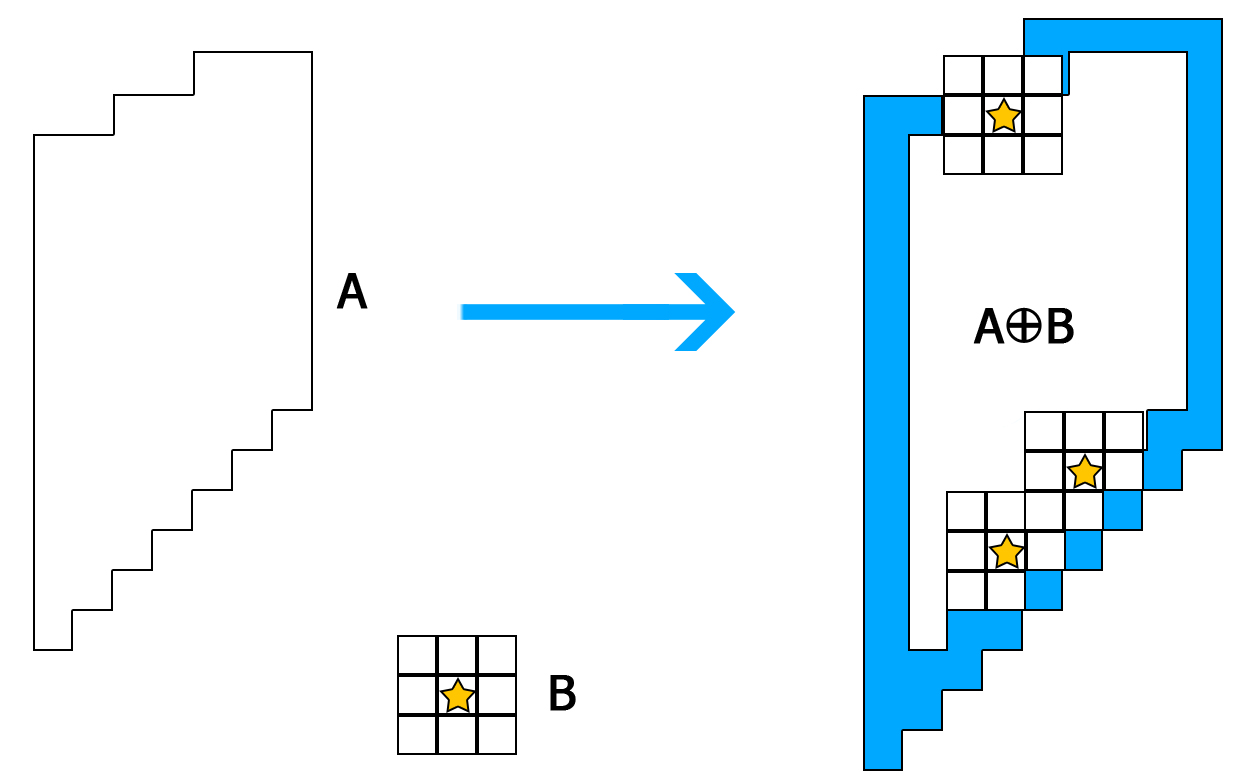
\includegraphics[scale=0.2]{imagenes/erosion-model.jpg}
\caption{Dilatación: A es la imagen original, B es el elemento estructurante, La estrella es el punto de referencia. Se ve como aumenta la imagen en proporci\'on al patr\'on aplicado }
\end{figure}

\subsubsection{Erosión}

La operación de erosión es análoga a la de dilatación, con la diferencia de que aplica el mínimo local en vez del máximo. Como resultado se obtiene una imagen más pequeña y oscura que la original \cite{BookOpenCv}. V\'ease en la figura \ref{fig:erosion}

\begin{figure}[hbtp]
\centering
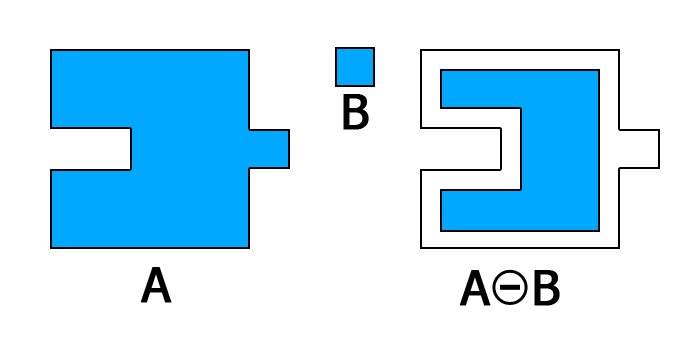
\includegraphics[scale=0.3]{imagenes/erosion.jpg}
\caption{Erosión,  A: es la imagen original, B: es el n\'ucleo, La estrella es el punto de referencia. Se ve como disminuye la imagen en proporci\'on al patr\'on aplicado}
\label{fig:erosion}
\end{figure}

%Este cap\'itulo constituyo la base te\'orica que sustenta el proyecto, en el siguiente cap\'itulo se presenta el proceso de desarrollo que se sigui\'o para su culminaci\'on. 
